\begin{figure}[h]
	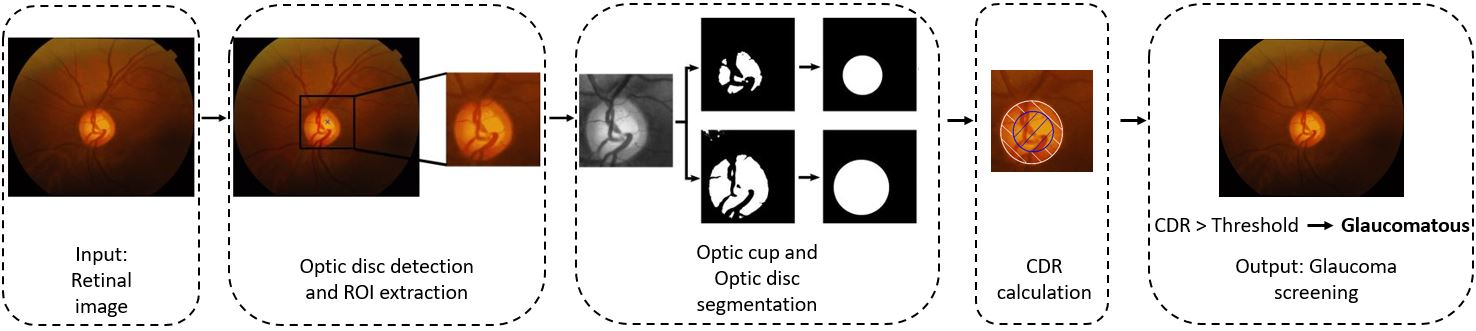
\includegraphics[width=\textwidth]{Images/full-image00.JPG}
	\caption{\label{diagramme}Flowchart of the proposed method for glaucoma screening and diagnosis.}
\end{figure}

The method for early glaucoma screening and diagnosis consists of the following main stages: optic disc (OD) detection and region-of-interest (ROI) extraction around the OD (see \mbox{section \ref{detection}}), optic cup (OC) and optic disc (OD) segmentation (see \mbox{section \ref{segmentation}}), cup-to-disc ratio (CDR) calculation (see \mbox{section \ref{cdr_calculation}}) and glaucoma screening (see \mbox{section \ref{glaucoma_screening}}). A flowchart of the proposed method is presented in \mbox{Fig. \ref{diagramme}}.
In this section, we also introduce the pseudo-codes of the proposed method for glaucoma screening, according to each stage of the algorithm. The written codes allow to stretch out the structure of the program, provide a complete understanding of the role of each function and create a bridge between the method and its implementation (\mbox{see Algorithms~\ref{alg:oddetection}, \ref{alg:detectbrightregions}, \ref{alg:templatematching}, \ref{alg:ocodsegmentation} and \ref{alg:glaucomascreening}).}


% ---------------------------- ONH Detection method ---------------------------------------- %

\subsection{\label{detection}Optic disc detection and ROI extraction}

%Text requiring further explanation\footnote{Example footnote}

OD detection is a primordial step in computer-aided systems, providing an essential contribution for the screening of diabetic \mbox{retinopathy (DR)} or glaucoma \citep{chrastek,dr}. However, automatic OD detection is a challenging task, particularly in the presence of bright lesions going with various ocular pathologies such as diabetic retinopathy, Coats disease, etc. \citep{xiong}. In \mbox{Fig. \ref{example_lesions}}, an example of this mentioned drawback is outlined. These bright lesions are not related to the glaucoma case, as glaucoma generates structural changes within the ONH only. Nevertheless, to ensure the glaucoma screening process, it is mandatory to ensure a robust OD detection, even if subjects eventually suffer from other diseases inducing the apparition of these bright lesions. Hence, we can reliably conduct glaucoma screening even in the presence of other ocular pathologies. 

\bigbreak

\begin{figure}[h]
\centering
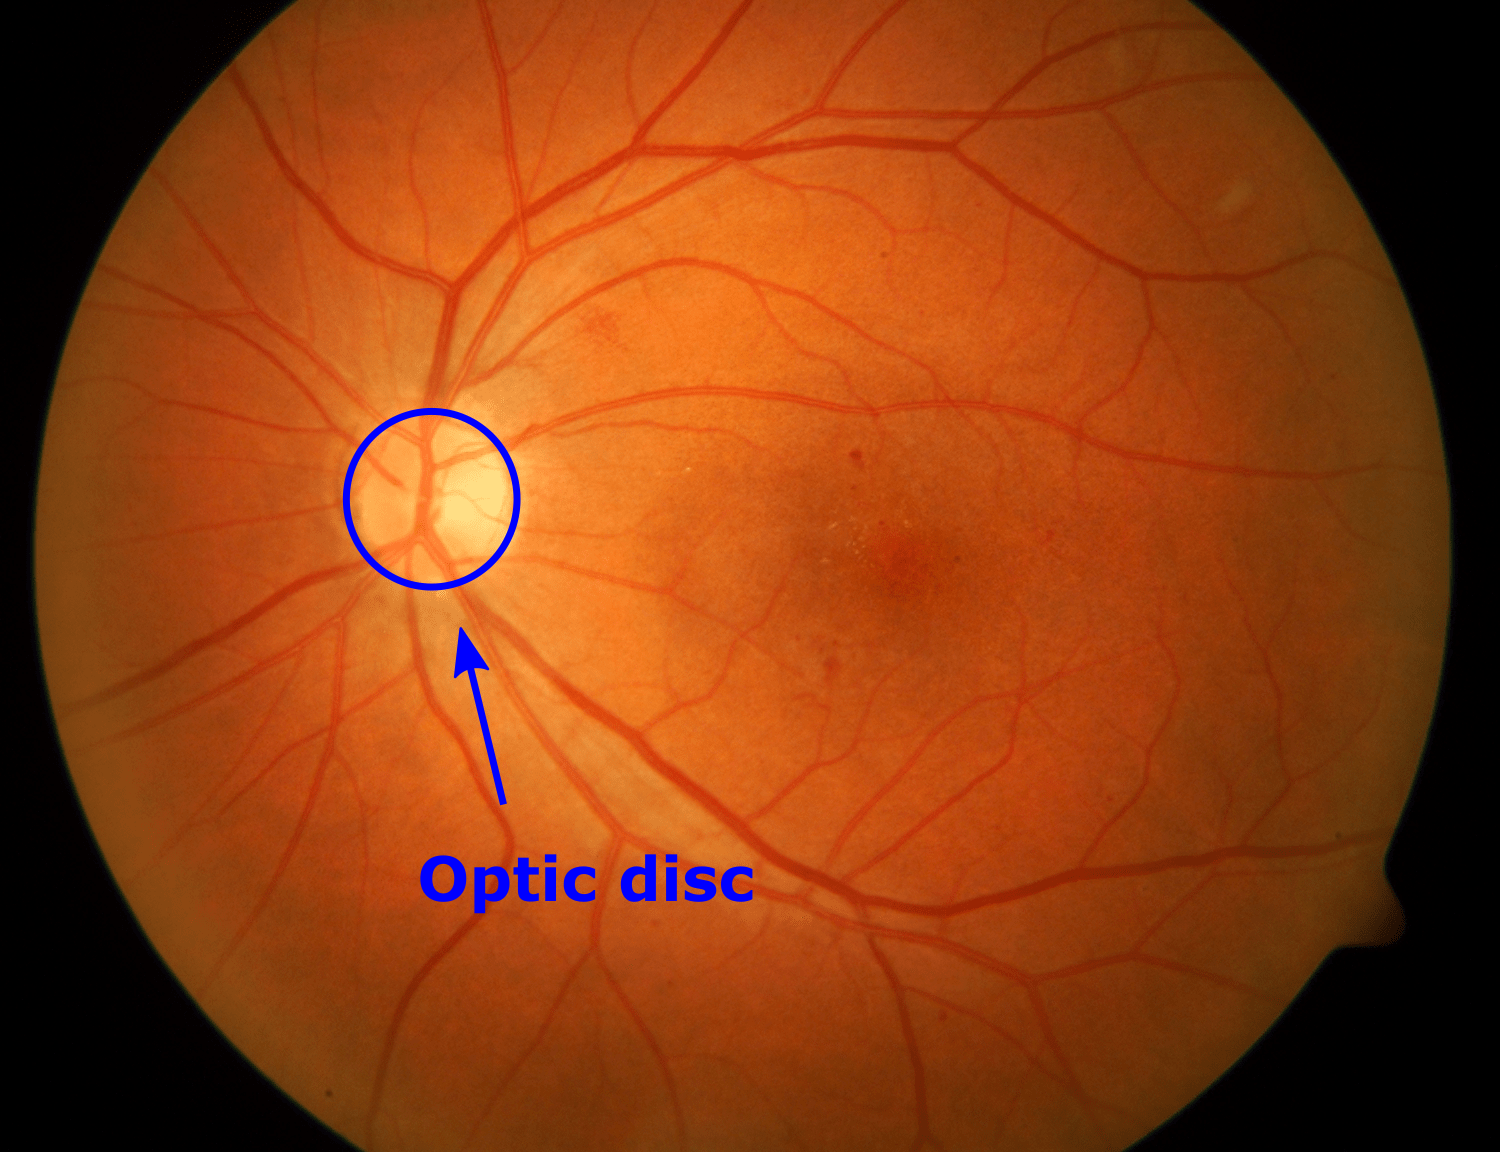
\includegraphics[width=4.5cm]{Images/Methode/Detection/examples/image006.png}{(a)}
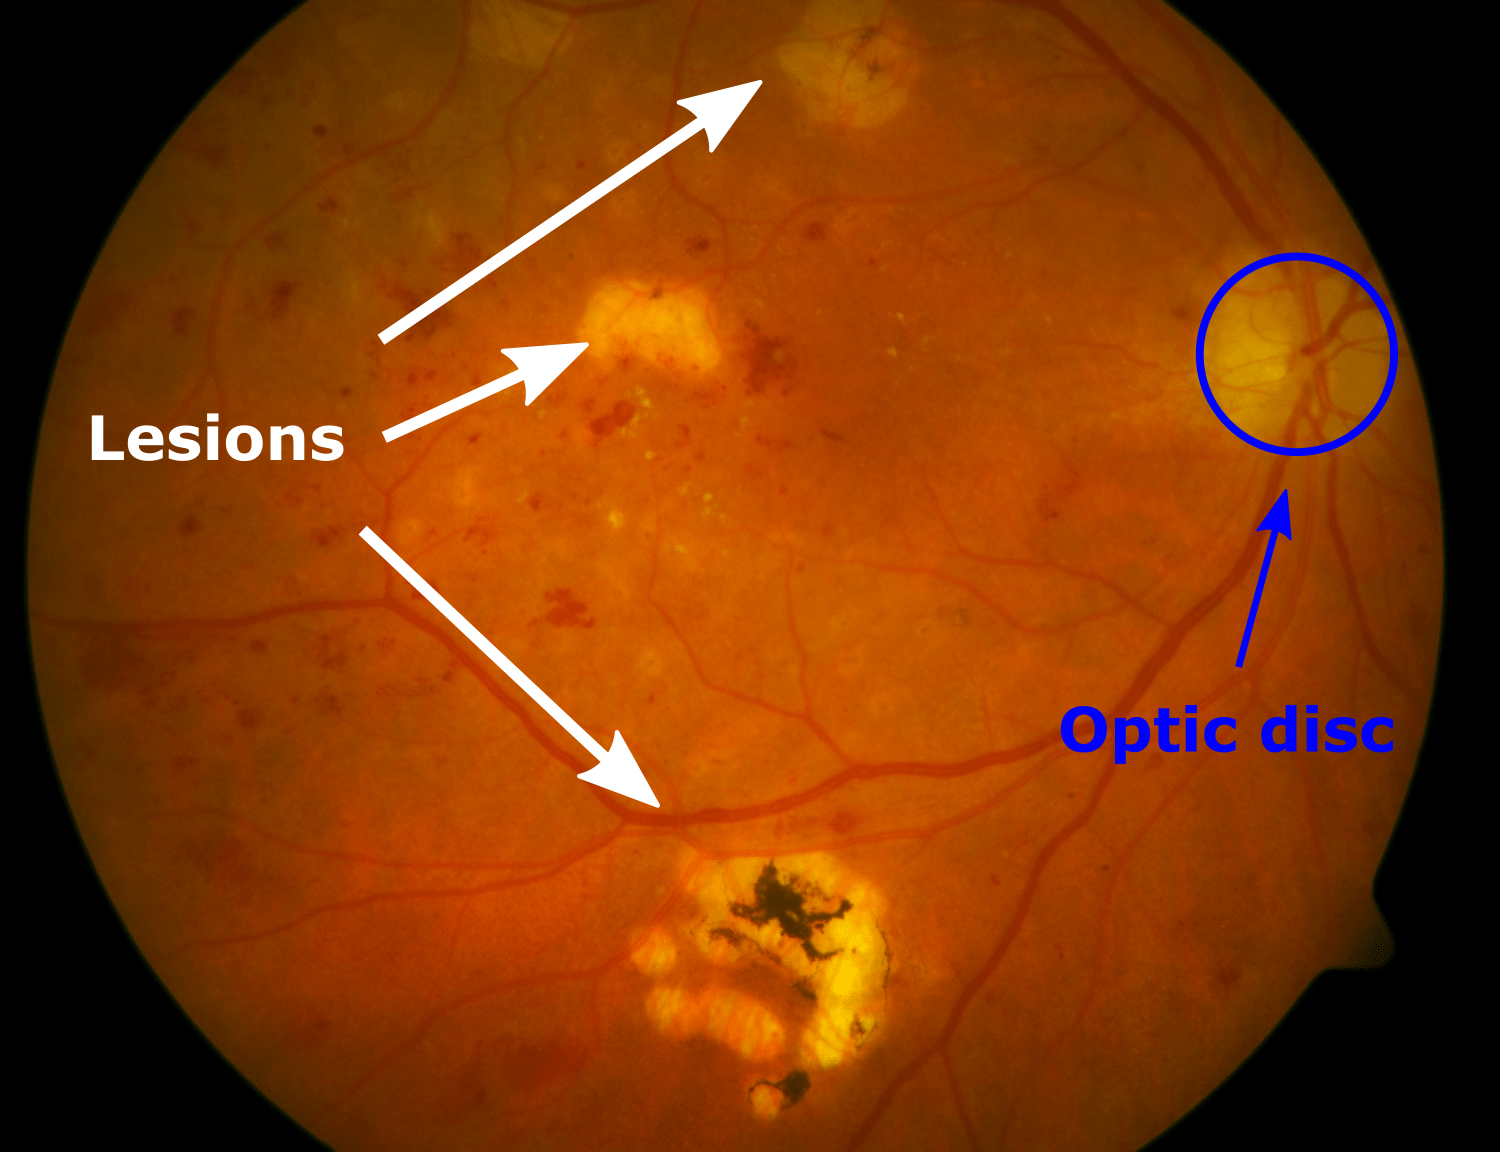
\includegraphics[width=4.5cm]{Images/Methode/Detection/examples/image_lesions.png}{(b)}

\caption{\label{example_lesions}Example with different retinal images: (a) retinal image without any lesion, (b) retinal image with large lesions, associated to a diabetic retinopathy.}
\end{figure}

Many approaches have been proposed in the literature for OD detection. They can be divided in three main categories: approaches based on vascular tree extraction, approaches based on OD appearance (brightness/circularity), and approaches based on OD template matching.

The approaches based on the vascular tree tend to extract the vessel structure and exploit its convergence to the OD center \citep{mahfouz,youssif,zhang}. \citet{foracchia} exploited the vessels direction using a geometrical model of the vascular structure, to detect the OD. \citet{soares} used the orientation of the four main vessels by computing cumulative sum fields, leading to OD center localization. These methods tend to be robust to the changes on OD appearance, and efficiently detect the OD in both healthy and pathological cases. However, a recent study \citep{sayadia2} showed that these approaches lead to an important computation complexity, as it requires a complete extraction of the retinal vascular tree. Hence, it is inappropriate to our study where the computational efficiency is an important parameter to consider. Also, the complete extraction of the vessels is challenging with obstructive lesions. 

To avoid the extraction of the vascular tree, some methods used the OD features such as brightness or circularity. It is the most intuitive feature to exploit, while bringing important information for OD detection. For example, \citet{pourreza} used the Radon transform \citep{radon} on several angles to detect bright and circular areas. Also, \citet{hashim} proposed a combination between morphological operations, and Gaussian differences that improves the edges visibility, to finally get the OD boundaries. \citet{rahebi} performed a high points intensity research, using a Firefly algorithm \citep{firefly}. In the work by \citet{giraddi}, a thresholding method is operated to extract bright areas, and an active contour algorithm lead to OD extraction. These methods tend to exhibit good results in healthy retinal images. However, they often suffer from some weaknesses with the presence of great-intensity lesions, and lower accuracy is observed compared to the methods based on the vascular tree (see \mbox{Fig. \ref{example_lesions} (b)} and \mbox{Fig. \ref{images_detect} (a)}).

OD Template Matching approaches tend to detect the OD in the image, from previously-defined OD models. The most relevant example of this approach is the work by \citet{dehghani}, which consists firstly of the creation of histogram models of the OD. Second, a scanning of the retinal image allows to detect the OD using a sliding sub-window and the computed model. On the same principle, \citet{wankhede} built an OD histogram model by estimating the OD radius, and computed a similarity coefficient between the OD histogram and current sliding sub-window to finally detect the OD final location.
Here, the main advantage compared to other approaches is that not any segmentation step is required. Also, these methods do not suffer from previously-exposed limitations, where they strongly depend on the OD appearance or on a complete extraction of the vessels. However, the main disadvantage is the entire image path to find the OD location, which can lead to eventual matching errors or more important computation times. 

\begin{algorithm}[h]
	
	\caption{OD detection}
	\label{alg:oddetection}
	{\fontsize{10}{9.5}\selectfont
	\begin{algorithmic}[1]
		
		\State \textbf{Input:} retinal image $I$ 
		\State \textbf{Output:} OD sub-image $OD\_crop$
		\medbreak

		\Function{od\_detection}{$I$}
			\State $centroids \gets$ \textsc{detect\_bright\_regions}$(I)$\Comment{see Algorithm 2}
			\If{$length(centroids) > 1$}
			\State $center \gets$ \textsc{template\_matching}$(od\_hist\_template, centroids, image)$\Comment{see Algorithm 3}
			\Else
			\State $center \gets centroids[0]$
			\EndIf
			\State $OD\_crop \gets I[center, S]$
			\State \textbf{return} $OD\_crop$
		\EndFunction
		
	\end{algorithmic}
	}
\end{algorithm}

We take into account each approach and its limitations and propose a new efficient and robust method for OD detection in retinal images \mbox{(see Algorithm~\ref{alg:oddetection})}. Several contributions are made in this work to provide a non computationally-complex method, while detecting the OD even in the presence of lesions. First, we detect the brightest regions in the retinal image (see \mbox{section \ref{detect_bright}}). Second, to effectively detect the final OD location among eventual bright lesions, a template matching technique is computed only on the found bright points (see \mbox{section \ref{template_matching}}). Finally, a sub-image around the OD is extracted.

\subsubsection{\label{detect_bright}Detection of bright regions}

Our approach for the detection of bright regions is composed of the following steps: preprocessing, thresholding, distance map computation and selection of the maximum points on the distance map \mbox{(see Algorithm~\ref{alg:detectbrightregions})}.

\begin{algorithm}[!htbp]
	
	\caption{Detection of the bright regions}
	\label{alg:detectbrightregions}
	{\fontsize{10}{9.5}\selectfont	
	\begin{algorithmic}[1]
		\State \textbf{Input:} retinal image $I$ 
		\State \textbf{Output:} list of coordinates $centroids$
		\medbreak
		
		\Function{detect\_bright\_regions}{$I$}
			\State $I \gets$ \textsc{histogram\_equalization}$(green\_level(I))$
			\State $binary \gets$ \textsc{otsu\_thresholding}$(I)$
			\State $map \gets$ \textsc{distance\_map}$(binary)$
			\For {all $p$ in $map$}
				\If{$p > max(map)/2$}
					\State $maxima[i,j] \gets 255$
				\Else
					\State $maxima[i,j] \gets 0$
				\EndIf
			\EndFor
			
			\For {all $convex\_component$ in $maxima$}
				\State $c \gets $\textsc{center\_of\_mass}$(convex\_component)$
				\State $centroids \gets centroids.append(c)$
			\EndFor
			\State \textbf{return} $centroids$
		\EndFunction
		
	\end{algorithmic}
	}
\end{algorithm}

First, since retinal images may suffer from some lighting defects, non-uniform intensity variations or poor contrast, a prior preprocessing step is computed \citep{hashim,youssif}. If color fundus images, green channel is extracted, since it provides the highest contrast and a better highlighting of the brightest regions in the retinal image \citep{inoue}.
Then, in order to enhance contrast and emphasize the visualization of the retinal structures, an adaptive histogram equalization method (CLAHE) \citep{pizer} is applied, offering a local-based contrast enhancement (see \mbox{Fig. \ref{images_detect} (b)}).

Thereafter, in order to efficiently separate needed bright regions to other retinal structures such as blood vessels or background, a binary thresholding method is operated. In this way, many methods exist and are applied for retinal image study, with global or local techniques \citep{soares}. Among this thresholding techniques, Otsu's local thresholding method appears as a best choice for this presented task, allowing good managing with uneven illumination when acquiring fundus images \citep{abramoff}.
Nevertheless, we notice that applying Otsu's method may lead to an inappropriate binarization in some extreme cases, separating the vascular tree from the other retinal components. To solve this problem, we set the obtained Otsu's threshold value $T_O$ to $(\frac{4}{3}) \times T_O$ to ensure the thresholding operation match with our context of detecting bright regions (see \mbox{Fig. \ref{images_detect} (c)}). An example with the applied function to separate the bright regions from background is presented in \mbox{Fig. \ref{threshold}}.


\begin{figure}[t]
	\centering
	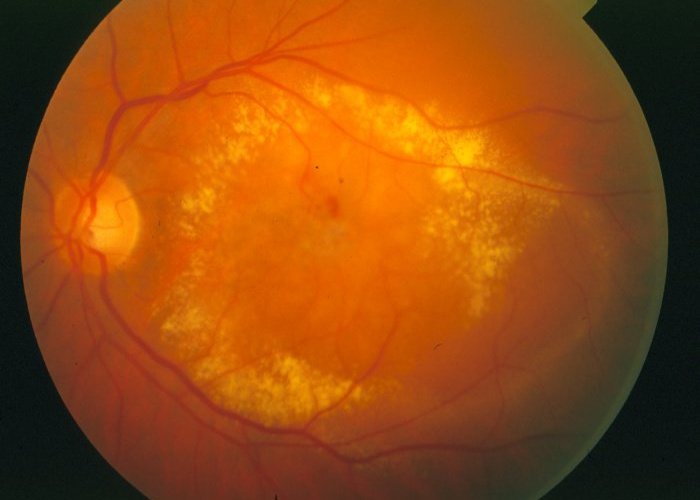
\includegraphics[width=4.0cm]{Images/Methode/Detection/im0002/im0002_.jpg}{(a)}
	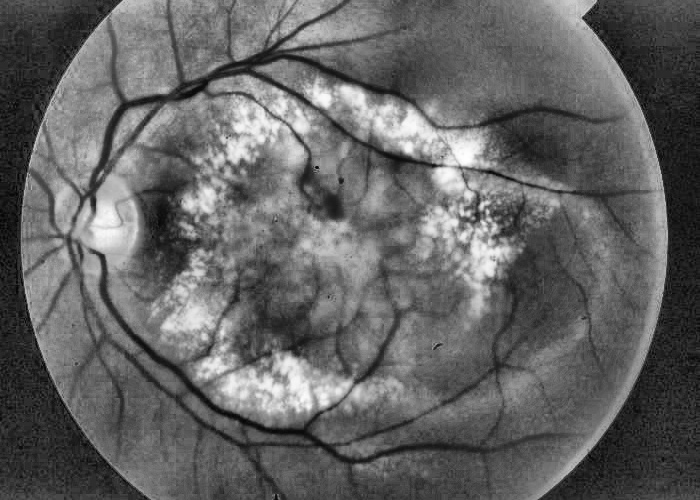
\includegraphics[width=4.0cm]{Images/Methode/Detection/im0002/1_image_egalisee.jpg}{(b)}
	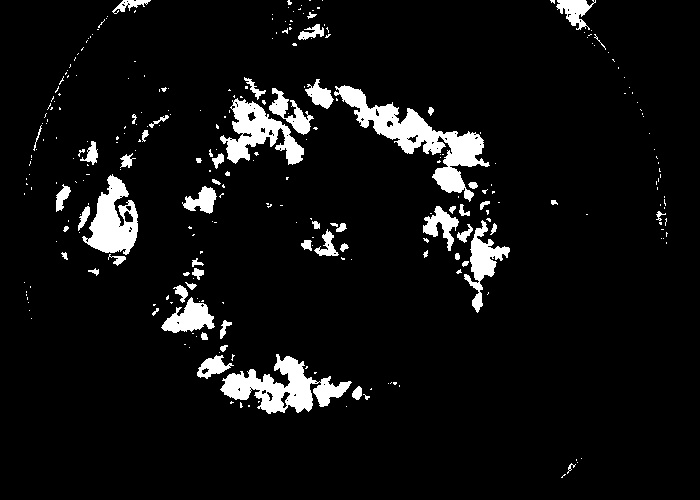
\includegraphics[width=4.0cm]{Images/Methode/Detection/im0002/2_image_seuillee.jpg}{(c)}\\
	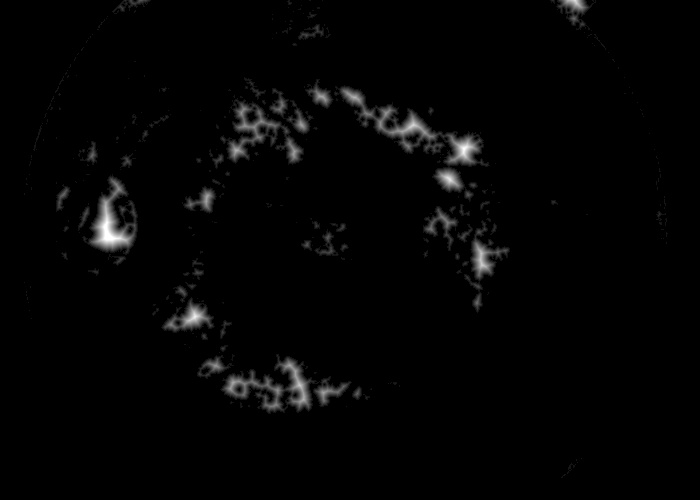
\includegraphics[width=4.0cm]{Images/Methode/Detection/im0002/3_image_dist.jpg}{(d)}
	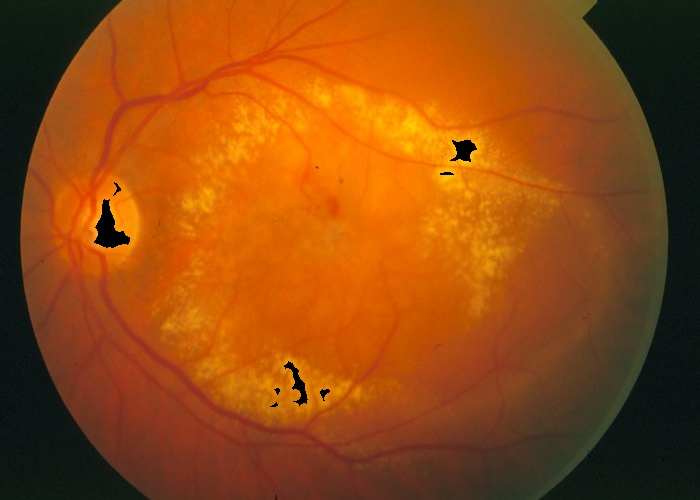
\includegraphics[width=4.0cm]{Images/Methode/Detection/im0002/4_image_points2.jpg}{(e)}
	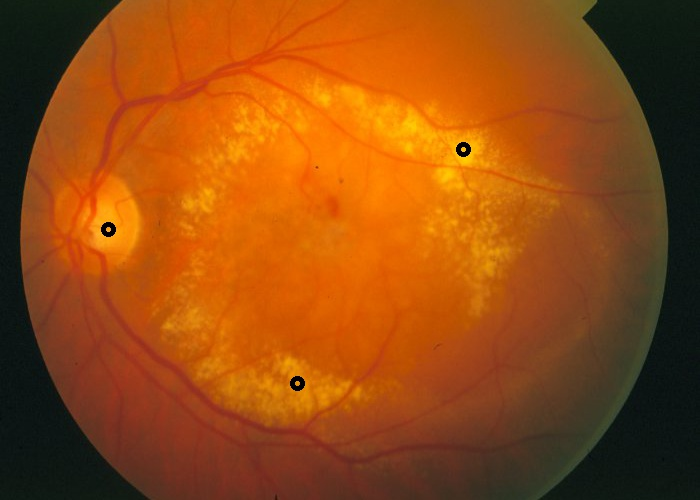
\includegraphics[width=4.0cm]{Images/Methode/Detection/im0002/points.jpg}{(f)}
	\caption{\label{images_detect}Detection of bright regions on a retinal image (STARE database): (a) Original retinal image with great-intensity lesions, (b) preprocessed image, (c) binary image, (d) distance map, (e) maximum points on distance map , (f) center approximation.}
\end{figure}


\begin{figure}[h]
    \centering
    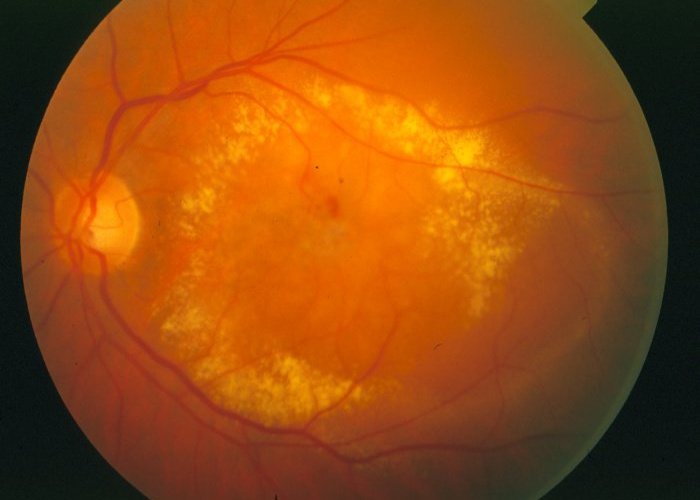
\includegraphics[width=3.5cm]{Images/Methode/Detection/im0002/im0002_.jpg}{(a)}
    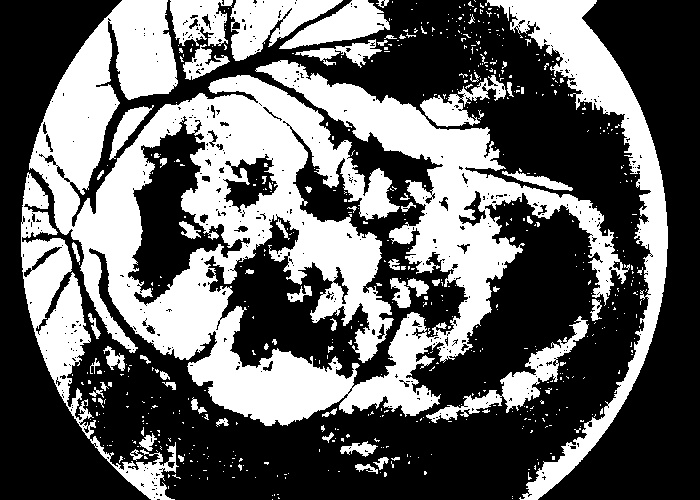
\includegraphics[width=3.5cm]{Images/Methode/Detection/im0002/image_seuillee.jpg}{(b)}
    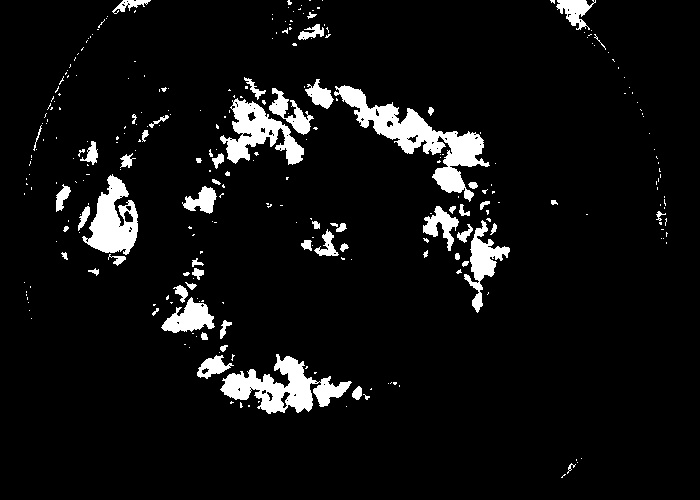
\includegraphics[width=3.5cm]{Images/Methode/Detection/im0002/2_image_seuillee.jpg}{(c)}
    \caption{\label{threshold}Example with applied thresholding method: (a) contrast-enhanced image, (b) binary image using Otsu's method, (c) final binary image applying supplement threshold value.}
\end{figure}

Then, to compute a derived metric representation of the obtained binary image, and emphasize all brightest areas, an intensity map is implemented. Here, the Euclidean distance map on the output binary image is applied: each white pixel is associated with its distance to the nearest black pixel \citep{xiong} (see \mbox{Fig. \ref{images_detect} (d)}).

Afterwards, in order to select the largest bright regions from the distance map, an adaptive selection is applied by extracting the interval $I = [\frac{1}{2} \times max_{DT}; \quad max_{DT}]$ depending on the maximum value $max_{DT}$ in the obtained distance map (see \mbox{Fig. \ref{images_detect} (e)}).
Finally, each area is replaced by its centroid, being a representative point of area location (see Fig. \mbox{\ref{images_detect} (f)}). 

\bigbreak

After these steps (preprocessing, thresholding, distance map computation, maximum points on distance map, center approximation), brightest regions are detected, each represented by its centroid as location point. 
In healthy cases, since no bright lesions are apparent, only one point is found then corresponds to the OD location. However, in the presence of bright lesions associated to pathological cases, other bright points may be detected. In this case, it is primordial to propose a complementary step for OD recognition, providing an efficient way to detect the OD location among eventual bright lesions. \mbox{Section \ref{template_matching}} presents the adopted strategy.

\subsubsection{\label{template_matching}Template Matching}

Here, we propose a template matching technique to detect the OD even in the eventual presence of bright lesions in the retinal image. The technique is in accordance with the strategy followed in \citet{dehghani,wankhede}. The two main steps of this technique are the creation of the OD histogram templates (see \mbox{section \ref{template_creation}}) and the matching among the found bright regions (see \mbox{section \ref{matching}}), finally leading to OD detection.

\paragraph{\label{template_creation}Creation of the OD histogram templates}


Here, we create the histogram templates associated to each evaluation database. We exploit well-known and often used databases for the evaluation of OD detection methods, such as DRIVE \citep{drive}, STARE \citep{stare}, DIARETDB0 \citep{diaretdb0}, DIARETDB1 \citep{diaretdb1} or ROC \citep{roc}. Since a representative OD model is required, several retinal images are chosen in the respective database (see \mbox{Fig. \ref{crop_hist} (a)}). Similarly to \citet{dehghani,osareh}, we make sure to use images with different OD appearance, to build the most robust OD model. 
For the following, each detailed step is applied to each chosen image.

\begin{figure}[t]
	\centering
	
	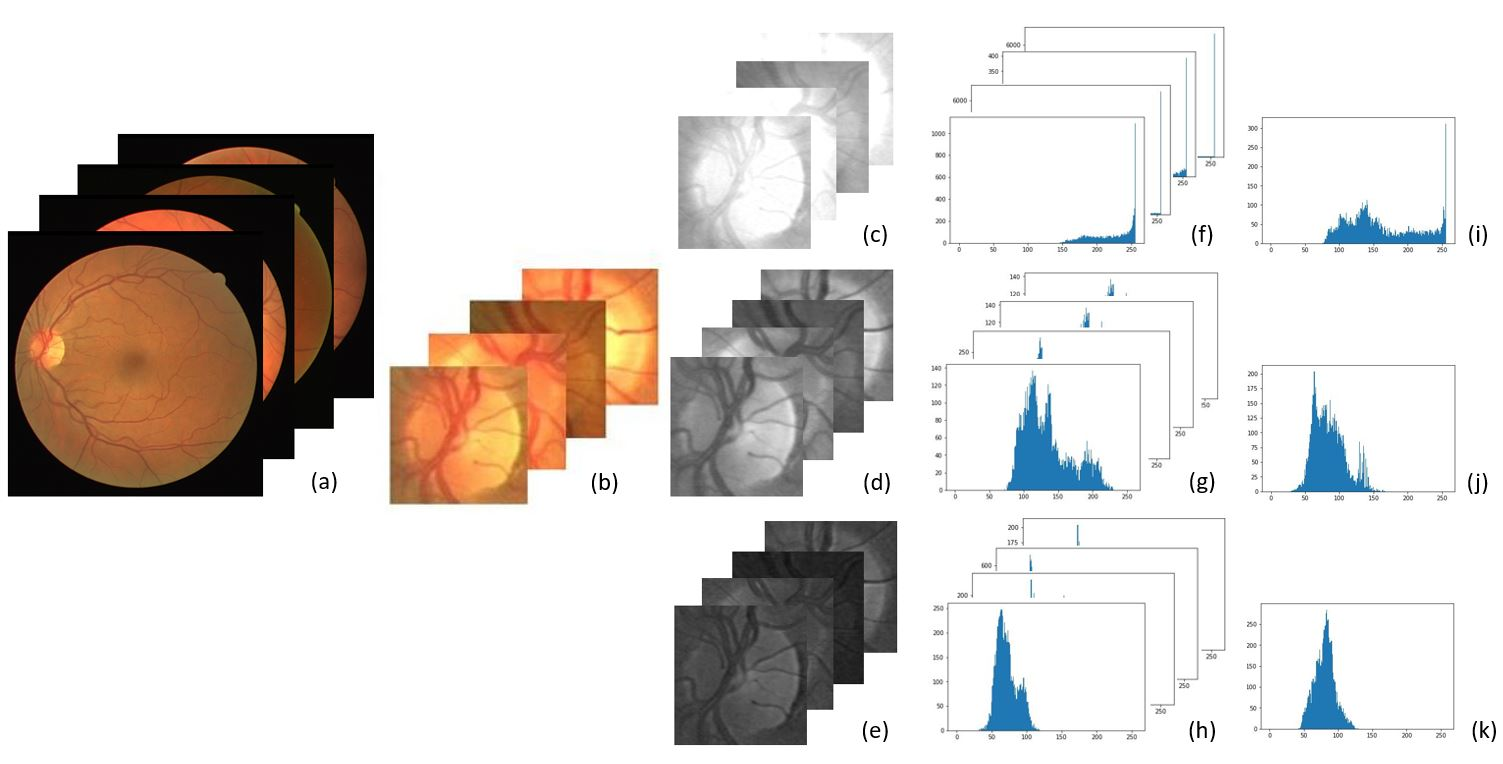
\includegraphics[width=0.9\textwidth]{Images/Methode/Detection/full-template.JPG}
	
	\caption{\label{crop_hist}Creation of the OD template, from the chosen retinal images to the template histograms (DRIVE database): (a) retinal images, (b) sub-windows around the OD, (c) red channel sub-windows, (d) green channel sub-windows, (e) blue channel sub-windows, (f) red channel histograms, (g) green channel histograms, (h) blue channel histograms, (g) mean red channel histogram, (h) mean green channel histogram, (i) mean blue channel histogram.}
\end{figure}


Firstly, since an OD model is needed, a sub-image around the OD is selected. Here, a semi-automatic extraction method is performed, using a manually-defined OD center and estimating automatically the OD radius \citep{wankhede}. Indeed, the OD radius (in pixels) in a retinal image depends on the intrinsic \mbox{Field-Of-View (FOV)} parameter of the used camera, and the resolution of the image. Let $N_{FOV}$ be the number of pixels in the FOV, and $A_{FOV}$ the specific area in the FOV. The image footprint, $I_{FP}$, is defined as:

\begin{equation}
I_{FP} = \frac{A_{FOV}}{N_{FOV}}
\label{footprint}
\end{equation}

\noindent So, the OD radius in pixels is calculated using the average human OD diameter \mbox{$D_{OD} \approx 1.85mm$} \citep{wankhede}. \mbox{Using (\ref{footprint})}, the OD radius $R_{OD}$ is defined as:

\begin{equation}
R_{OD} =  \sqrt[]{\frac{(D_{OD}/2)^2}{I_{FP}}}
\label{rayon_disque}
\end{equation}

\noindent Using (\ref{rayon_disque}), automatic estimation of the square length $l$ of the sub-image
is defined as:
\begin{equation}
l = 2 \times R_{OD} + \Delta
\label{square_length}
\end{equation}

\noindent with $\Delta = \nicefrac{1}{3} \times R_{OD}$ to make sure to contain all the OD in the sub-image.

\begin{table}[h]
\small
\centering

\begin{tabular}{|c|c|c|c|c|}
\hline
\textbf{Dataset} & \textbf{$A_{FOV}$} ($mm^2$)& \textbf{Image size} ($N_{FOV}$) & \textbf{$R_{OD}$} & \textbf{ROI ($l$)} \\
\hline
DRIVE \citep{drive} & 124.8 & 768 x 584 & 55 & 75 \\
\hline
STARE \citep{stare} & 235.6 & 605 x 700 & 125 & 165 \\
\hline
DIARETDB0 \citep{diaretdb0} & 54.3 & 1500 x 1152 & 165 & 220 \\
DIARETDB1 \citep{diaretdb1} & {} & {} & {} & {} \\
\hline
ROC \citep{roc} & 37.4 & 1386 x 1391 & 210 & 280 \\
%{} & {} & {} & {} & {} \\
%{} & {} & 768 x 576 & {} & {} \\
%\hline
%VARIA \cite{varia} & 25* & 768 x 584 & 100 & 130 \\
\hline
\end{tabular}

\caption{\label{tableau_fov}$R_{OD}$ values for several retinal images on the publicly available datasets, and computed $ROI$ square length.}
\end{table}

\mbox{Table \ref{tableau_fov}} presents the value of the obtained OD radius obtained from different image databases, using described parameters and formulas. Using these results and setting up the OD center, the approximation of the OD radius allows to extract the sub-image around the OD from each selected images (see \mbox{Fig. \ref{crop_hist} (b)}).


Then, in order to exploit all the information provided by the color image, the three red, green and blue channels are extracted from the sub-image. If the method for OD detection is applied on gray-scale images, we use the gray-scale channel only (see \mbox{Fig. \ref{crop_hist} (c), (d) and (e)}).

Afterwards, the histogram for each extracted sub-image is computed then registered, as it provides relevant trend of intensity values present in the calculated OD sub-image (see \mbox{Fig. \ref{crop_hist} (f), (g) and (h)}).

Finally, we gather the resulting histograms of each chosen images for the template creation, and compute the associated mean histogram to each extracted channel. Here, three final histogram templates are obtained for color images, among the chosen images (see \mbox{Fig \ref{crop_hist} (i), (j), (k)}). Otherwise, in gray-scale images, one histogram is obtained, corresponding to the mean histogram computed on the gray-scale sub-images.

\paragraph{\label{matching}Matching}

\begin{algorithm}[!htbp]

	\caption{Template matching}
	\label{alg:templatematching}
	{\fontsize{10}{9.5}\selectfont
	\begin{algorithmic}[1]
		\State \textbf{Input:} retinal image $I$, list of coordinates $centroids$, histogram template $od\_hist\_template$ 
		\State \textbf{Output:} Coordinates of the OD $OD\_coordinates$
		\medbreak
		
		\Function{template\_matching}{$I$}

			\For {all $c$ in $centroids$}
				\State $crop \gets image[c, s]$\Comment{crop around the point $c$, with square size $s \times s$}
				\State $hist \gets$ \textsc{calcul\_hist}$(crop)$
				\State $corr \gets$ \textsc{correlation}$(hist, od\_hist\_template)$					
				\If{$corr > max\_corr$}
					\State $max\_corr \gets corr$
					\State $center \gets c$
				\EndIf
			\EndFor
			\State \textbf{return} $OD\_coordinates$
		\EndFunction
		
	\end{algorithmic}
	}
\end{algorithm}


After the creation of the OD histogram templates, matching phase is applied on the found bright regions (see \mbox{section \ref{detect_bright}}) to detect the final OD location \mbox{(see Algorithm~\ref{alg:templatematching})}.

First, from the position of each detected bright region in the image (see \mbox{section \ref{detect_bright}}), we extract a surrounding sub-image centered on each detected point position. The square length is automatically set using the same technique as described in \mbox{Eq. (\ref{square_length})}. 

After, if exist, the channels are separated, giving for each point position three sub-images in color images or one sub-image in gray-scale images. Then, the histogram of each sub-image is computed as described in \mbox{section \ref{template_creation}}.

Next, to launch template matching and final OD detection, cross-correlation method is performed between the histogram templates, and the associated histograms to each bright point. The Correlation Similarity Index between two histograms $a$ and $b$ is defined as:

\begin{equation}
c = \frac{1}{(1 + \sum_{n}(a_k - b_k)^2)}
\label{corr}
\end{equation}

\noindent where $k$ denotes the histogram bins, and for two similar histograms, $\sum_{n}(a_k - b_k)^2 \approx 0$ and $c \approx 1$.

For gray-scale images, we \mbox{use (\ref{corr})} to compute the correlation between the two gray-scale histograms. For color images, we use a weighted sum function. The correlation between the histograms is defined then as:

\begin{equation}
C(i,j) = \alpha \times c_R + \beta \times c_G + \gamma \times c_B
\label{corr2}
\end{equation}

\noindent with $(i,j)$ the coordinates of the central window point, $c_{\lambda}$ the Correlation Similarity Index of the histograms of each color channel $\lambda = R, G, B$, and $\alpha$, $\beta$, $\gamma$ positive weights allowing to master the influence of each channel. Since the green channel provides a better contrast, when blue and even more red channels may suffer from non-uniform OD illumination or more artifacts \citep{hashim}, weights are defined as $\alpha = 0.5$, $\beta = 2$ and $\gamma = 1$ to enhance green channel influence \citep{dehghani}. 

Finally, the retained OD location point is associated to the window with the highest correlation value between the corresponding histogram and the employed template one, among all found bright points (see \mbox{section \ref{detect_bright}}).

An example of the template matching result is illustrated in \mbox{Fig. \ref{exemple_tm}}, with the found bright regions (see \mbox{Fig. \ref{exemple_tm} (a)}), and the final OD location result after applying the template matching. An extraction of the sub-window around the OD location represents the region-of-interest (ROI) (see \mbox{Fig. \ref{exemple_tm} (c)}).

\bigbreak

\begin{figure}[h]
    \centering
    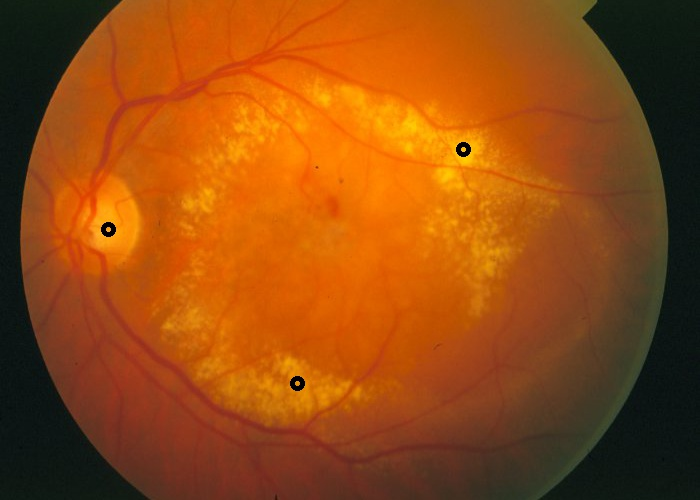
\includegraphics[height=3cm]{Images/Methode/Detection/im0002/points.jpg}{(a)}
    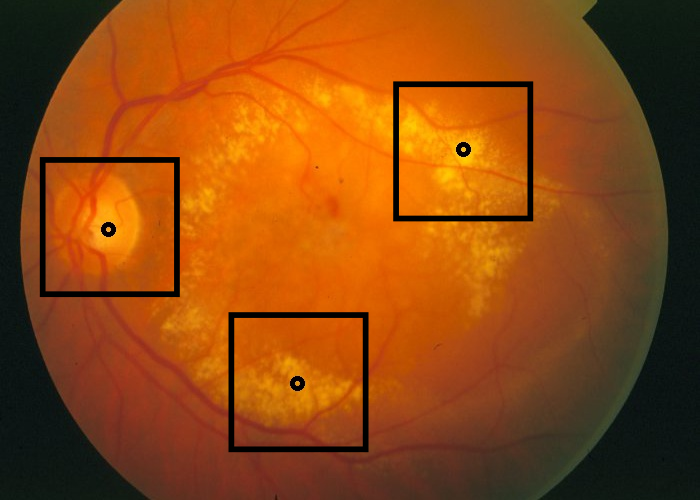
\includegraphics[height=3cm]{Images/Methode/Detection/im0002/framed_points2.png}{(b)}
    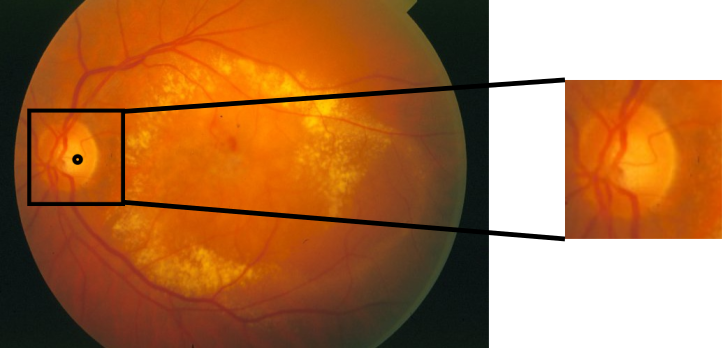
\includegraphics[height=3cm]{Images/Methode/Detection/im0002/final_crop.png}{(c)}
    \caption{\label{exemple_tm}Template Matching on detected bright points: (a) image with the detected points, (b) image with framed neighborhood around the points, (c) final OD location point with the extracted ROI.}
\end{figure}

\bigbreak

We note that our new proposed OD detection method ensures a robust and effective ROI extraction around the OD, even in the potential presence of bright lesions going with pathological cases. 
%These bright lesions are not related to the glaucoma case, but to other ocular diseases coming forward in the retina. However, it is primordial to discard these eventual bright lesions and effectively conduct glaucoma screening, when subjects eventually suffer from other ocular diseases such as diabetic retinopathy.
To compute the CDR and lead to glaucoma screening from the extracted ROI sub-image, a joint OC-OD segmentation method is proposed in \mbox{section \ref{segmentation}}.

% ----------------------------- OC and OD segmentation --------------------------------- %

\subsection{\label{segmentation}Optic cup and optic disc segmentation}

\begin{algorithm}[h]
	
	\caption{OC and OD segmentation}
	\label{alg:ocodsegmentation}
	{\fontsize{10}{9}\selectfont
	\begin{algorithmic}[1]
		
		\State \textbf{Input:} OD sub-image $OD\_crop$
		\State \textbf{Output:} OC segmentation $optic\_cup$, OD segmentation $optic\_disc$
		\medbreak
		
		\Function{oc\_od\_segmentation}{$OD\_crop$}
		\State $gray\_level \gets$ \textsc{gray\_level}$(OD\_crop)$
		\State $image\_kmeans, label, centers \gets$ \textsc{k-means}$(gray\_level, 4)$ \label{kmeansoperation}
		\State $maximum \gets max(centers)$
		\State $second \gets second(centers)$
		\State $first\_label \gets label[maximum]$
		\State $second\_label \gets label[second]$
		\medbreak
		\For {all $p$ in $image\_kmeans$}
			\If{$label(p) == first\_label$}
				\State $optic\_cup[p] \gets 255$
			\ElsIf{$label(p) == second\_label$}
				\State $optic\_disc[p] \gets 255$
			\EndIf
		\EndFor
		\medbreak
		\For{$image$ in ${optic\_cup, optic\_disc}$}
			\State $circle \gets$ \textsc{circular\_hough\_transform}$(image)$ \label{houghoperation}
			\For{p in $image$}
				\If{$p$ in $circle$ and $p == 0$}
					\State $p \gets 255$
				\ElsIf{$p$ outside $circle$ and $p == 255$}
					\State $p \gets 0$
				\EndIf
			\EndFor
		\EndFor
		\medbreak
		\State \textbf{return} $optic\_cup$, $optic\_disc$
		\EndFunction
		
	\end{algorithmic}
	}
\end{algorithm}

OC and OD segmentation plays a key role in many computer-aided diagnosis systems in ophthalmology. It is an essential task to identify ocular conditions such as glaucoma or diabetic retinopathy \citep{cheng,nugraha}.
Nevertheless, the segmentation of the OC and even more the OD is difficult, since they have not well-defined boundaries.

As viewed with the related works for glaucoma screening (see \mbox{section \ref{related_work}}), existing methods for OC and OD segmentation are ranged into supervised or unsupervised approaches.
When supervised methods require a constraining training phase, with important resources and computationally-complex algorithms, unsupervised approaches bring a slighter computation cost. Hence, we follow this lane to deliver an easy-to-perform method from 2-D retinal images.
However,  a lack on the segmentation performance is noticed with existing unsupervised approaches, what influences the obtained CDR value and final glaucoma screening. 

To overcome the lacks of existing methods, we present a new effective approach for joint OC-OD segmentation \mbox{(see Algorithm~\ref{alg:ocodsegmentation})}. Here, the main challenge is to establish a trade-off between segmentation rate and computation efficiency. In this way, we firstly perform a texture-based method, relying on the intensity aspect of the areas, to give a prior segmentation of the required areas. Secondly, a model-based boundary fitting method allows to properly detect the edges, smoothing the borders and improving the segmentation result.
Starting from the gray-level sub-image of the OD (see \mbox{section \ref{detection}}), the proposed segmentation method consists of the two following steps: texture-based pixel classification (see \mbox{section \ref{pixel_classification}}) and model-based boundary fitting (see \mbox{section \ref{boundaries_detection}}).

\subsubsection{\label{pixel_classification}Texture-based pixel classification}

To compute the joint OC-OD segmentation, a texture-based strategy is firstly operated to classify each pixel among a retinal structure. Here, an unsupervised clustering approach is adopted, to avoid a learning phase and its resource-intensive process. K-means clustering is a well-known classification algorithm, which consists in grouping similar points following a nearness criterion \citep{kmeans}. A well-defined distance \mbox{function $D(x,y)$} and a positive \mbox{integer $K$} are the two parameters for K-means clustering. Frequently, the used \mbox{distance $D$} is the Euclidean distance \citep{kodinariya}. The \mbox{value $K$} is often related to the context, and corresponds to the number of clusters needed to find. From \mbox{$K$ cluster} centroids, using the \mbox{distance $D$}, each data point is allocated to the cluster of the nearest centroid.

In this segmentation context, where texture is a relevant feature to extract and show off each retina component, the K-means clustering algorithm is employed using an intensity-based nearness criterion. Thus, this approach allocates each area of the retinal sub-image among \mbox{$K$ clusters} following its gray-level. Since the main retinal components are the OC, the OD, the background and the blood vessels, a fixed \mbox{value $K = 4$} is selected.
\mbox{Fig. \ref{kmeans}} presents an example of the applied clustering method with different values \mbox{of $K$}. \mbox{For $K = 2$} (see \mbox{Fig. \ref{kmeans} (b)}), we notice that there is a separation between the entire OD area and the retinal area, without a distinction between the OC and the OD. Inversely, too much areas appear \mbox{for $K = 8$} (see \mbox{Fig. \ref{kmeans} (d)}). This result strengthens the choice of the \mbox{value $K = 4$} (see \mbox{Fig. \ref{kmeans} (c)} and \mbox{Fig. \ref{etapes_segmentation} (b)}). 

\begin{figure}[t]
 \centering
 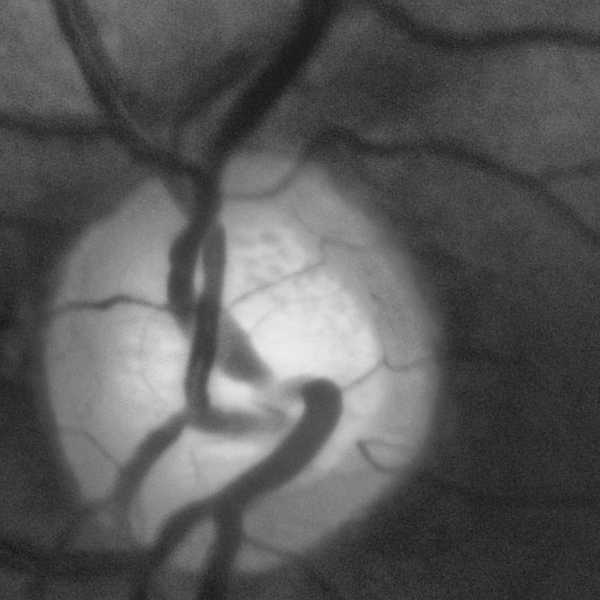
\includegraphics[width=2.5cm]{Images/Methode/Segmentation/0_crop.png}{(a)}
 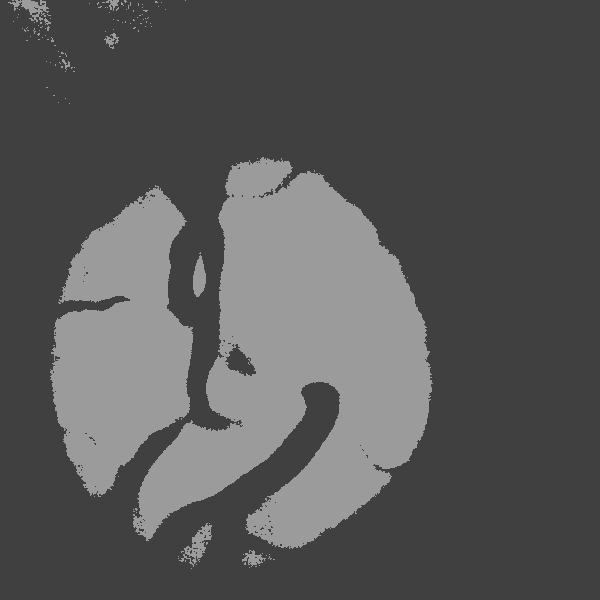
\includegraphics[width=2.5cm]{Images/Methode/Segmentation/Kmeans/clustering2.png}{(b)}
 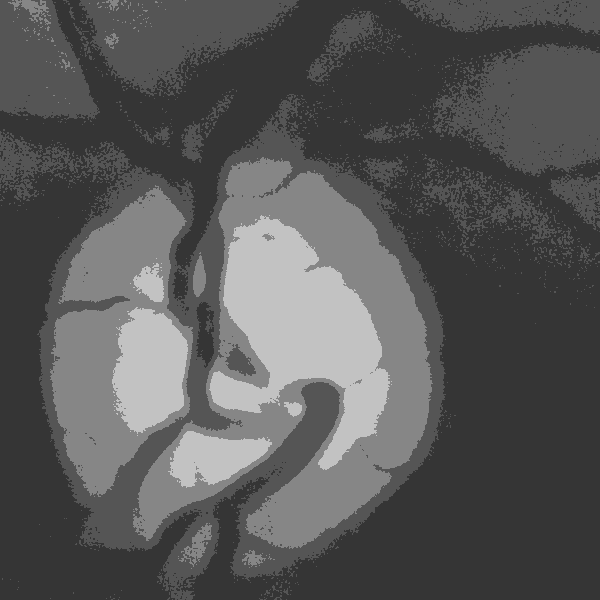
\includegraphics[width=2.5cm]{Images/Methode/Segmentation/1_kmeans.png}{(c)}
 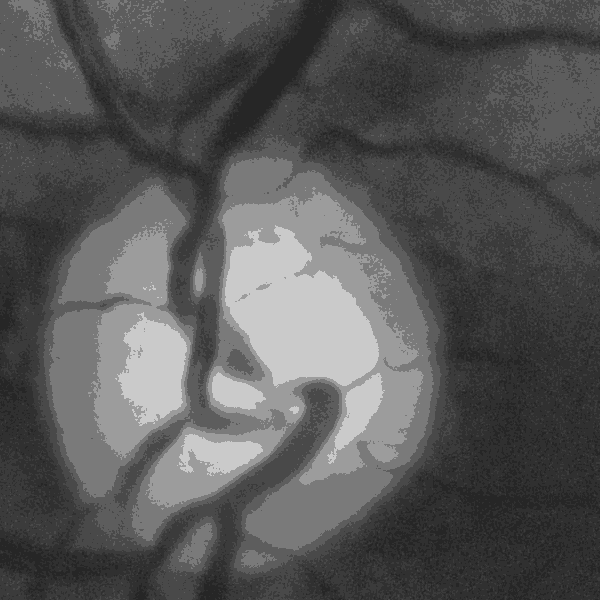
\includegraphics[width=2.5cm]{Images/Methode/Segmentation/Kmeans/clustering8.png}{(d)}
 \caption{\label{kmeans} Applied clustering method on input OD sub-image: (a) OD gray-level sub-image, (b) K-means with K=2, (c) K-means with K=4, (d) K-means with K=8.}
 
\end{figure}

Then, since the OC and the OD are the greater-intensity areas in the sub-image, they are both associated to the two greater-intensity clusters. Thus, the cluster with the greater intensity corresponds to the OC area, when the second greater-intensity cluster corresponds to the Neuro-Retinal Rim (NRR) area. The gathering of each found area forms the OD.
From this result, to obtain an uniform rendering, the output K-means image is further thresholded twice using respectively the greater-intensity and the second greater-intensity (see \mbox{Fig. \ref{etapes_segmentation} (c) and (d)}).

\subsubsection{\label{boundaries_detection}Model-based boundary fitting}

From the segmentation result after applying the pixel classification (see \mbox{section \ref{pixel_classification}}), some gaps are apparent on both OC and OD areas because of the presence of the blood vessels converging into the OD. Also, some noise along the borders is present, which can degrade the segmentation accuracy.
Since morphological operators may not always fill in these gaps, with variable blood vessels thicknesses, a strategy consists in computing a fitting of both OC and OD boundaries. This fitting strategy also allows to smooth the OC and OD borders, while improving the segmentation accuracy \citep{wong}. Here, since regions of interest are known for their rather circular feature, circular Hough transform \citep{pedersen} is performed \citep{aquino,zhu}. 
After detecting the OC and OD borders by applying the circular Hough transform, we consider that each pixel inside the circle is part of the final segmentation, and final segmentation is unaltered by the presence of the blood vessels (see \mbox{Fig. \ref{etapes_segmentation} (e) and (f)}).

\begin{figure}[t]

    \centering
    \renewcommand{\arraystretch}{2}
    
    \begin{tabular}{p{2.5cm} p{2.5cm} p{2.5cm} p{2.5cm}}
        
        {} & {} & \multirow{2}{*}{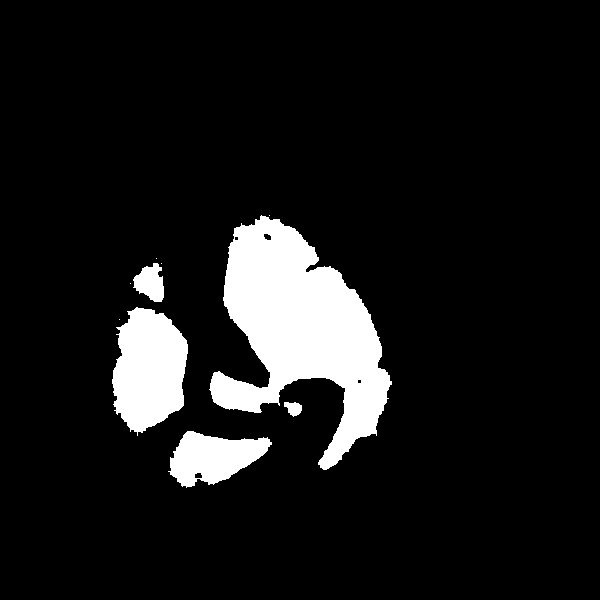
\includegraphics[width=2.5cm]{Images/Methode/Segmentation/2_cup.png}{(c)}} & 
        \multirow{2}{*}{
\includegraphics[width=2.5cm]{Images/Methode/Segmentation/6_hough_cup.png}{(e)}} \\
        
        \multirow{2}{*}{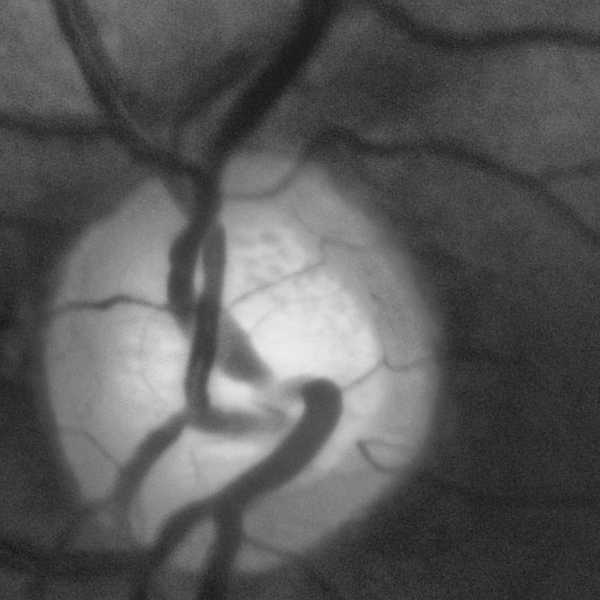
\includegraphics[width=2.5cm]{Images/Methode/Segmentation/0_crop.png}{(a)}} & 
        \multirow{2}{*}{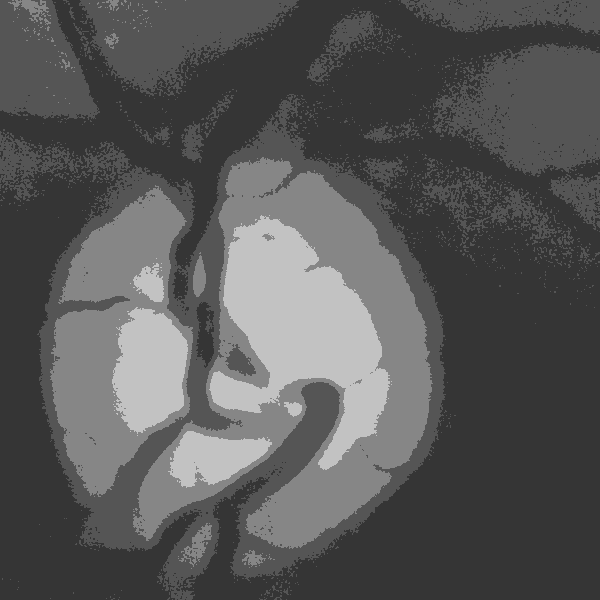
\includegraphics[width=2.5cm]{Images/Methode/Segmentation/1_kmeans.png}{(b)}} & {} & {} \\
        
        {} & {} & \multirow{2}{*}{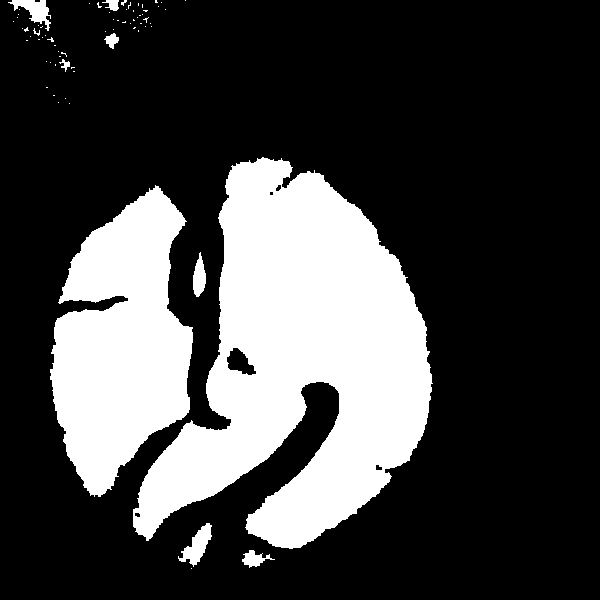
\includegraphics[width=2.5cm]{Images/Methode/Segmentation/3_do.png}{(d)}} & 
        \multirow{2}{*}{
\includegraphics[width=2.5cm]{Images/Methode/Segmentation/7_hough_do.png}{(f)}} \\
        
        {} & {} & {} & {} \\
    
    \end{tabular}
    
    \caption{\label{etapes_segmentation}Example with OC and OD segmentation method steps: (a) sub-image around the OD, (b) k-means with K=4, (c) OC extraction and thresholding, (d) OD extraction and thresholding, (e) final OC segmentation, (f) final OD segmentation.}
    
\end{figure}


Within our new proposed method for joint OC-OD segmentation, OC and OD areas are extracted on the retinal image. Texture-based feature followed by model-based fitting allow to effectively segment each desired area. For the further, CDR calculation is proposed in \mbox{section \ref{cdr_calculation}} for glaucoma screening.

\subsection{\label{cdr_calculation}CDR calculation}

Many methods have exploited the relevant cup-to-disc ratio (CDR) feature for early glaucoma screening. The CDR is a reliable clinical feature to estimate the structural changes of the ONH, and assess an early-occurring glaucoma. In this context, two different forms of CDR exist and are exploited in state-of-the-art approaches, both assessing the cupping of the ONH and being factors of glaucoma presence risk \citep{cdr}.
First, the diameter-based CDR consists in computing the ratio between the vertical (or horizontal) diameter of each OC and OD regions. This feature have been extensively used in state-of-the-art methods, well-accepted by specialists \citep{cheng}.
Second, recent methods for early glaucoma screening and diagnosis have used the area-based CDR, $CDR_{area}$ \citep{nugraha, priyadharsini}. $CDR_{area}$ consists in the ratio between the area of each OC and OD regions:

\begin{equation}
    CDR_{area} = \frac{OC_{area}}{OD_{area}}
\end{equation}

\noindent where each area is defined as the number of pixels in each respective region. Area-based CDR provides a 2-D feature-based measurement allowing to assess the structural changes of the ONH \citep{maldhure}.  Hence, we adopt this choice as it appears as a better criteria for our glaucoma screening context aiming to measure the cupping portion onto the ONH. In this way, from each OC and OD segmentation (see \mbox{section \ref{segmentation}}), we calculate their respective area (number of white pixels), to finally compute the area-based CDR and conduct to glaucoma screening \mbox{(see Algorithm~\ref{alg:glaucomascreening})}.

\begin{algorithm}[!htbp]

	\caption{Glaucoma screening}
	\label{alg:glaucomascreening}
	{\fontsize{10}{9}\selectfont
	\begin{algorithmic}[1]
		\State \textbf{Input:} OC segmentation $optic\_cup$, OD segmentation $optic\_disc$
		\State \textbf{Output:} Glaucoma diagnosis $diag$
		\medbreak
		
		\Function{glaucoma\_screening}{$optic\_cup, optic\_disc$}
		
		\State $area\_oc \gets$ \textsc{area\_calculation}$(optic\_cup)$
		\State $area\_od \gets$ \textsc{area\_calculation}$(optic\_disc)$
		\State $CDR \gets \frac{area\_oc}{area\_od}$
		\medbreak
		\If{$CDR > 0.63$}
			\State $diag \gets$ 'Glaucomatous'
		\Else
			\State $diag \gets$ 'Healthy'
		\EndIf
		\medbreak
		\State \textbf{return} $diag$
		\EndFunction
		
	\end{algorithmic}
	}
\end{algorithm}

Using CDR calculation, glaucoma screening strategy is proposed in \mbox{section \ref{glaucoma_screening}}.

\subsection{\label{glaucoma_screening}Glaucoma screening}

In this section, we present the approach for glaucoma screening and diagnosis, using the CDR feature.
To achieve this required classification between healthy and glaucomatous subjects, many techniques are employed by existing glaucoma screening methods using different classifiers to assign the retinal images among their actual class \citep{singh2}.
One of the most popular glaucoma classifier is the Support Vector Machine (SVM), a supervised classification method which determinates a maximum-margin among the features to separate the classes \citep{maheshwari}. An other well-known classification method for glaucoma screening is the \mbox{$k$-Nearest Neighbor classifier ($k$-NN)}, a supervised method which associate each data to the predominant class of its \mbox{$k$ closest} neighbors (with $k$ a positive integer) \citep{bock}.
In these two supervised methods, several features need to be extracted in addition to the CDR to feed the supervised algorithm and improve the classification accuracy. Moreover, the choice of these features is challenging \citep{joshi}.

CDR-based methods generally classify each retinal image using a binary classification method. It consists in the use of a soundly-chosen thresholding value $T$. Thus, using the computed CDR, a simple binary classification is operated. A CDR value lower than the threshold value  $T$ agrees with a healthy subject, otherwise, it corresponds to a glaucomatous subject \citep{cheng,singh2,yin}. 
In our work, this simple approach is used, providing more ease and less computational cost while trustworthiness in final glaucoma screening and diagnosis. Indeed, exploiting the CDR clinical factor involves more reliability and efficiency on the final classification, while avoiding the use of hardly-chosen image-based features for a greedy learning phase. Here, the challenge is to set a reliable threshold value, allowing to effectively separate healthy subjects from glaucomatous ones.
To set up the accurate threshold value according to the CDR values within each healthy and glaucomatous class, we choose to compute the threshold value $T$ depending on the mean $\bar{m}$ and standard deviation $\sigma$ of the obtained CDR values of each retinal images among healthy and glaucomatous classes in the annotated \mbox{database (see \mbox{Eq. \ref{T}})}. 
%From the obtained CDR value of each retinal image, the threshold \mbox{value $T$} will depend on the \mbox{mean $\bar{m}$} and standard \mbox{deviation $\sigma$} values among each healthy ($H$) and glaucomatous ($G$) classes:

\begin{equation}
    \bar{m_H}+\sigma_{H} \quad < \quad T \quad \leq \quad \bar{m_G}-\sigma_{G}
    \label{T}
\end{equation}

\noindent where $\bar{m_H}$ and $\bar{m_G}$ are respectively the mean of healthy and glaucomatous computed CDR, and $\sigma_{H}$ and $\sigma_{G}$ are respectively the standard deviation of the healthy and glaucomatous computed CDR.
\bigbreak

After proposing a complete methodology for glaucoma screening from fundus images, used materials and obtained experimental results of the proposed method are expressed in the following section.
